% ======================================================================
\chapter[INTRODUCTION \& PROJECT FORMULATION]{Introduction \& Project Formulation}
\label{ch:intro}
% ======================================================================

\section{Overview}

Magnetic resonance imaging (MRI) is widely used to examine the soft tissues of the knee, such as the ligaments, menisci and cartilage, which plain X-ray images do not show well \cite{bien2018}. A single knee study contains several image series. Each series is a stack of thin slices taken in one of three planes with one of several pulse sequences. A radiologist reads all of them and writes a free-text report that states which structures are torn, worn, swollen or bruised.

This project builds a deep learning system that reads a complete knee MRI study, exactly as it comes out of the scanner in DICOM format, and gives a probability for each of twelve abnormalities. The work was carried out on the data of the RSNA Knee Abnormality Detection challenge, a public machine learning competition hosted on Kaggle by the Radiological Society of North America (RSNA) \cite{kaggle_rsna_knee,rsna2026announce}. The competition provided a large multi-centre dataset and a test set whose labels were hidden from all teams. Because of this, the leaderboard gave an independent check of the design decisions we made.

\subsection{Clinical background}

The knee joint is formed by the femur, the tibia and the patella. Its stability depends on four main ligaments, two of which, the anterior cruciate ligament (ACL) and the medial collateral ligament (MCL), are among the findings studied here. Two C-shaped pads of fibrocartilage, the medial and lateral menisci, sit between the femur and the tibia and spread the load across the joint. The joint surfaces are covered with articular cartilage, and its gradual loss is called osteoarthritis (OA). Radiologists describe OA separately for the medial and lateral tibiofemoral compartments and for the patellofemoral (PF) compartment behind the kneecap.

Besides these structural findings, a report usually comments on the fluid inside the joint (an effusion), on thickening and inflammation of the joint lining (synovitis), on a fluid-filled Baker's cyst behind the knee, and on the bones themselves, which can show a bruise (bone contusion) or a fracture after trauma. Some of these findings are focal and visible on two or three slices, such as a meniscal tear. Others, such as an effusion, are spread over a large part of the joint. A useful system therefore has to look at the right part of the right series for each finding.

A knee MRI study is acquired in three planes. Sagittal slices are stacked from one side of the knee to the other, and each shows a front-to-back view in which the cruciate ligaments and the menisci are seen along their length. Coronal slices are stacked from front to back and show the collateral ligaments and the medial and lateral compartments side by side. Axial slices are horizontal and show the patellofemoral joint and the fluid pockets around it. Each plane is usually imaged with a fluid-sensitive, fat-suppressed sequence, in which fluid and oedema appear bright, and often also with a sequence without fat suppression that shows anatomy more clearly.

\subsection{The RSNA knee abnormality detection challenge}

The task set by the organisers is to predict, for each test study, the probability that each of the twelve findings in Table~\ref{tab:targets} is present. The study is the unit of prediction: there is one row per study in the submission file, whatever the number of series it contains.

\begin{table}[htbp]
\centering\footnotesize\setstretch{1}
\caption[The twelve findings and their gold-58 positives]{The twelve findings predicted by the system, with the competition's definitions and the number of positive studies among the 58 expert-labelled training studies}
\label{tab:targets}
\begin{tabular}{L{3.2cm}L{8.4cm}C{2.2cm}}
\toprule
Target column & Definition used by the organisers & Positives in gold-58 \\
\midrule
ACL & anterior cruciate ligament injury & 24 \\
MCL & medial collateral ligament injury & 9 \\
Medial Meniscus & tear of the medial meniscus & 26 \\
Lateral Meniscus & tear of the lateral meniscus & 23 \\
Medial OA & osteoarthritis of the medial tibiofemoral compartment & 15 \\
Lateral OA & osteoarthritis of the lateral tibiofemoral compartment & 11 \\
PF OA & patellofemoral osteoarthritis & 21 \\
Effusion & joint effusion (excess fluid in the joint) & 35 \\
Synovitis & inflammation of the joint lining & 27 \\
Baker's & Baker's (popliteal) cyst & 12 \\
Contusion & bone contusion (bone bruise) & 19 \\
Fracture & fracture & 18 \\
\bottomrule
\end{tabular}
\end{table}

\paragraph{Evaluation metric.} Submissions are scored with the macro-averaged area under the receiver operating characteristic curve (ROC-AUC) \cite{hanley1982,fawcett2006}. For a finding $k$, the AUC is the probability that a randomly chosen positive study receives a higher score than a randomly chosen negative study,
\begin{equation}
\auc_k=\frac{1}{|P_k|\,|N_k|}\sum_{i\in P_k}\sum_{j\in N_k}\Big[\mathbf{1}(\hat p_{ik}>\hat p_{jk})+\tfrac12\,\mathbf{1}(\hat p_{ik}=\hat p_{jk})\Big],
\label{eq:auc}
\end{equation}
where $P_k$ and $N_k$ are the positive and negative test studies for that finding, $\hat p_{ik}$ is the predicted probability, and $\mathbf{1}(\cdot)$ is one when its condition holds and zero otherwise. The competition score is the plain mean over the twelve findings,
\begin{equation}
S=\frac{1}{12}\sum_{k=1}^{12}\auc_k .
\label{eq:macroauc}
\end{equation}
Because the AUC depends only on the order of the scores, the metric does not reward calibrated probabilities or a good choice of threshold. It rewards ranking the positive studies above the negative ones, separately for every finding. A rare finding such as MCL injury counts exactly as much as a common one such as effusion.

\paragraph{Training data.} The training set contains 4,407 knee MRI studies with their DICOM files and one radiology report per study. Only 58 of these studies carry expert labels for all twelve findings. We call them the \emph{gold-58} set throughout this report. The other 4,349 studies have a report and nothing else. The reports are written in nine languages and were produced in routine clinical work, so they follow each hospital's habits rather than a fixed template. Reports are not available for test studies. They can be used to create training labels, but the model itself has to work from the images alone.

\paragraph{Test data and rules.} The hidden test set has about 1,300 studies. It is swapped in only when a submitted notebook is scored, so participants never see it. The competition was run as a \emph{code competition}: a submission is a Kaggle notebook that must read the raw test DICOMs and write the predictions within nine hours of run time, with internet access switched off. Freely and publicly available external data and pretrained models were allowed. Each team could make five submissions per day and select two final submissions for the private leaderboard. The data licence allows research use but forbids passing the data on to anyone outside the competition \cite{kaggle_rsna_knee}. Apart from one workstation screenshot of a public example study, this report therefore shows statistics and diagrams rather than MRI images from the dataset. These rules (nine hours, no internet, five submissions a day, no redistribution) are referred to in later chapters without being repeated.

\subsection{Characteristics of the dataset}

Before any modelling we audited the full dataset: every series, every DICOM header and every report. The main numbers are collected in Table~\ref{tab:dataset} and Figure~\ref{fig:dataset}.

\begin{table}[htbp]
\centering\footnotesize\setstretch{1}
\caption{Summary of the training data, measured over all files in our audit}
\label{tab:dataset}
\begin{tabular}{L{7.2cm}L{6.8cm}}
\toprule
Quantity & Value \\
\midrule
Studies (gold-labelled / report only) & 4,407 (58 / 4,349) \\
Series / DICOM files / size on disk & 24,371 / 819,078 / 569~GB (uncompressed) \\
Series per study & median 5 (range 3--14) \\
Slices per study & median 162 (range 67--632) \\
Studies with all three planes & 4,407 (100\%) \\
Fluid-sensitive series missing & sagittal 257, coronal 159, axial 0 studies \\
Laterality tag present in the DICOM header & 2,204 studies (50\%) \\
Report languages & 9 (English, Spanish, Turkish, Croatian, Greek, German, Bulgarian, Dutch, French) \\
Patient identifiers & pseudonymised per study (4,407 unique) \\
Pixel-identical duplicate studies & 1 pair, with two conflicting reports \\
\bottomrule
\end{tabular}
\end{table}

\begin{figure}[htbp]
\centering\setstretch{1}
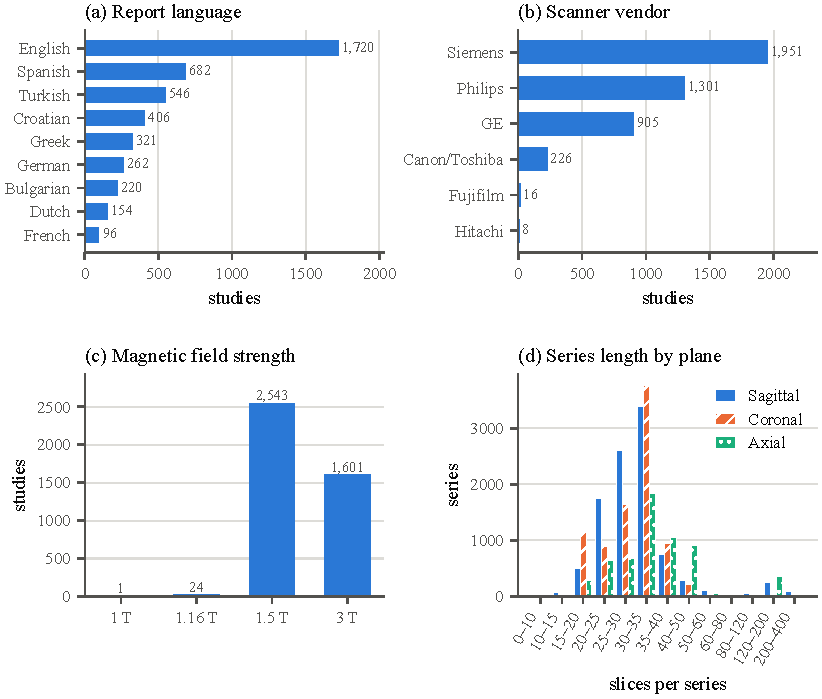
\includegraphics[width=\textwidth]{fig_dataset.pdf}
\caption[Composition of the training studies]{Composition of the 4,407 training studies: (a) report language, (b) scanner vendor, (c) field strength where the header records it, and (d) the number of slices per series in each plane}
\label{fig:dataset}
\end{figure}

Several of these properties shaped the project from the start. Language, hospital and scanner vendor are tied together: all Bulgarian studies come from Philips scanners, and all German, Greek and Dutch studies from Siemens scanners. Raw intensity values differ by a factor of about 25 between vendors, so no fixed intensity window can be used. Almost every study has more than one sagittal series, and some three-dimensional acquisitions contain up to 320 slices, while a typical two-dimensional series has about 30 slices that are 3--4~mm apart. A 512-pixel image may cover anything from 120 to 200~mm, so the physical size of a pixel varies between studies.

The orientation of the images also matters. In the coronal and axial planes, a right knee shows its lateral side on the left of the image and a left knee shows it on the right. A model that is not told which knee it sees has to learn every medial and lateral finding twice. The DICOM laterality tag is present for only about half of the studies, but we found that the side can be recovered for every series from the patient coordinates stored in the header, with 97.8\% agreement with the tag where both exist.

The gold-58 set is also unusual. Every gold study has at least one positive finding, with 4.1 positives per study on average, so the set contains no normal knees. Participants in the competition reported that these labels came from radiologists reading the images rather than the report. We could not confirm this from an official source. Our own measurements in Chapter~3 agree with it, because the reports leave out about half of the synovitis that the gold labels mark as present.

\subsection{Existing systems}

\paragraph{Deep learning on knee MRI.} Deep learning for knee and other joint MRI has been surveyed in a recent scoping review \cite{fritz2022review}. The best known earlier system is MRNet \cite{bien2018}. It was trained on 1,370 knee examinations from Stanford University Medical Center and predicts three labels: any abnormality, ACL tear and meniscal tear. MRNet runs a two-dimensional convolutional network (AlexNet) on every slice of a series, takes the maximum of the slice features, and combines the three planes with logistic regression. On its own hospital's data it reached an AUC of 0.965 for ACL tears, but on an external dataset of 917 examinations from a hospital in Croatia the same model scored 0.824 before it was retrained \cite{bien2018,stajduhar2017}. A model can learn the habits of one site, and this matters here because the competition data comes from many sites and scanners.

Other public knee datasets serve different purposes. The KneeMRI dataset of {\v S}tajduhar \emph{et al.} \cite{stajduhar2017} grades ACL injury on sagittal volumes from one Croatian hospital. fastMRI \cite{zbontar2018fastmri} was built for image reconstruction from raw scanner data, and fastMRI+ \cite{zhao2022fastmriplus} later added pathology annotations to part of it. The Osteoarthritis Initiative (OAI) \cite{nevitt_oai} is a long-term cohort study with MRI and expert grading of knee osteoarthritis. None of these datasets covers the twelve findings of this task with one consistent set of labels.

\paragraph{Learning from study-level labels.} A study-level label says that a finding is present somewhere in the study but does not say on which slice. Multiple-instance learning (MIL) treats the study as a bag of instances (slices or groups of slices) with one label for the whole bag. Attention-based MIL \cite{ilse2018} learns a weight for each instance and pools the instance features with these weights. The weights are learned from the bag label alone and often point to the instances that carry the finding. This idea is the core of the image model developed in this project.

\paragraph{Image encoders.} A convolutional neural network (CNN) applies small learned two-dimensional filters to an image, much like a bank of FIR filters applied along two axes, and stacks many such layers with non-linear functions between them so that later layers respond to larger and more complex patterns. Training such a network from scratch needs far more labelled images than medical datasets usually have. The usual practice is therefore to start from a network that was \emph{pretrained} on a large collection of natural photographs such as ImageNet \cite{deng2009imagenet}, and then \emph{fine-tune} it, that is, continue training all its weights on the medical task. EfficientNet \cite{tan2019effnet,tan2021effnetv2} and ConvNeXt \cite{liu2022convnext} are two widely used families, and CoAtNet \cite{dai2021coatnet} mixes convolution with attention. Self-supervised encoders such as DINOv2 \cite{oquab2024dinov2} produce general features that can be used without training the encoder at all. We tried frozen encoders first and fine-tuned encoders later; Chapter~3 shows why the second approach was necessary.

\paragraph{Labels from radiology reports.} When images have no labels but have reports, the reports can be turned into labels. For chest X-rays, the CheXpert labeller \cite{irvin2019chexpert} used hand-written rules with explicit uncertainty classes, and CheXbert \cite{smit2020chexbert} replaced the rules with a trained language model. VisualCheXbert \cite{jain2021visualchexbert} then showed that labels read from reports disagree substantially with labels read from the images by radiologists, and that a report labeller trained to match image-based labels agrees better with radiologists who read the images. In this report we call labels of the second kind \emph{image-read labels}. Large language models (LLMs) such as the Qwen family \cite{qwen2025qwen25,yang2025qwen3} can read reports in many languages without task-specific training, which makes them attractive for multilingual data like ours.

\paragraph{Approaches in the competition.} Many teams shared notebooks and label sets during the competition. The strongest public notebooks used two-dimensional encoders on stacks of three neighbouring slices (a ``2.5D'' input), pooled over slices and series with attention, and trained on labels extracted from the reports with LLMs. The highest public scores also relied on models trained with extra knee MRI data from the OAI. After the competition the top teams published their methods, and the first- and seventh-placed teams released their label sets and, in the first case, their code \cite{tascj_boxpool,songqizhou_llmlabels}; Section~\ref{sec:impl-post} describes what we took from them.

\paragraph{Gap addressed by this project.} Existing published systems either predict a few findings, depend on thousands of expert labels, or were developed on a single site. The competition data offers the opposite situation: many findings, many sites and languages, and almost no expert labels. The project therefore had to solve two problems together, the labelling problem and the image modelling problem, and had to evaluate both without a large, trusted labelled set.

\subsection{Problem statement}

Given a knee MRI study as a folder of DICOM files, estimate the probability of each of the twelve findings in Table~\ref{tab:targets}, using a model trained on 4,407 studies of which only 58 have expert labels and the rest have free-text reports in nine languages. The system must run offline on a single Kaggle GPU within nine hours for about 1,300 studies, must not use report text at prediction time, and must be evaluated in a way that does not overstate its accuracy.

\section{User Requirement Analysis}

The system has three kinds of users, and each brings its own requirements.

The first ``user'' is the competition's scoring service. It runs our notebook on the hidden test set and expects a correctly formatted file. Its requirements are strict and fully specified: one row per test study, twelve probability columns, no missing values, a run time below nine hours, and no internet access. The test DICOMs may also be compressed with JPEG-Lossless or JPEG~2000, which the local copy of the data never was, so the system must decode both.

The second group is the project team. We needed to run experiments on one laptop with a 6~GB graphics card and on Kaggle's free GPUs, compare ideas fairly, and repeat any result later. For us the important requirements were reproducibility, honest evaluation and the ability to restart long jobs after interruptions.

The third group is the audience of the final demonstration: faculty members, radiology researchers and fellow students who want to see what the model does with a study and why. They need a simple way to load a study, to see the findings with their probabilities, and to see which part of the image drove each prediction. The system must not suggest that it is fit for clinical use.

Table~\ref{tab:requirements} lists the requirements that followed from this analysis, with the section that describes how each was handled.

\begin{table}[htbp]
\centering\footnotesize\setstretch{1}
\caption{Functional (F) and non-functional (N) requirements of the system}
\label{tab:requirements}
\begin{tabularx}{\textwidth}{l Y L{2.4cm}}
\toprule
ID & Requirement & Met in \\
\midrule
F1 & Read a study as raw DICOM files, including JPEG-Lossless and JPEG~2000 compressed files, and order slices by their position in space & \S\ref{sec:impl-mil}, \S\ref{sec:testing} \\
F2 & Produce twelve probabilities per study in the competition's submission format & \S\ref{sec:impl-mil}, \S\ref{sec:impl-post} \\
F3 & Handle missing or unreadable series without silently inventing image data & \S\ref{sec:impl-mil}, \S\ref{sec:testing} \\
F4 & Turn multilingual reports into training labels for all 4,349 unlabelled studies & \S\ref{sec:impl-audit} \\
F5 & Show the predictions and the image evidence behind them for a single study & \S\ref{sec:impl-demo} \\
N1 & Run offline on one Kaggle T4 GPU within nine hours for about 1,300 studies & \S\ref{sec:impl-mil}, \S\ref{sec:impl-post} \\
N2 & Train and run on a laptop GPU with 6~GB of memory & \S\ref{sec:impl-mil}, \S\ref{sec:impl-demo} \\
N3 & Keep competition data on our machines; no report text sent to hosted services & \S\ref{sec:impl-audit}, \S\ref{sec:impl-demo} \\
N4 & Do not select our own models on the 58 gold studies; report uncertainty with confidence intervals (not followed for the last-day blends of Stage~4) & \S\ref{sec:method-eval}, \S\ref{sec:impl-endgame} \\
N5 & Make every reported number traceable to a script, a log or a leaderboard entry & \S\ref{sec:testing}, Appendix \\
\bottomrule
\end{tabularx}
\end{table}

\section{Feasibility Study}

\paragraph{Technical feasibility.} The full training data takes 569~GB uncompressed, and one study contains about 160 slices. A frozen-feature model can be trained on any machine once the features are cached, but a model that fine-tunes its image encoder must decode and process images on every training step. We had a laptop with an Intel Core i5-13420H processor, 32~GB of memory and an NVIDIA RTX~4050 Laptop GPU with 6~GB of memory. A pilot run showed that a ConvNeXt-Tiny encoder on 224-pixel inputs, with three series and eight slice windows per study, needs 3.8~GB of GPU memory and about seven minutes per epoch on this laptop, which made local training possible. Kaggle provides two NVIDIA T4 GPUs with 15~GB each for 30 hours a week per account, which was enough for larger models later in the project. Local inference of our own model took about 1.9~s per study, or about 42 minutes for 1,300 studies, well within the nine-hour limit.

\paragraph{Economic feasibility.} All software used in the project is open source, and all the compute came from the team's own laptop and the free weekly Kaggle GPU quota of our accounts. We also asked for a small GPU quota on a commercial cloud as a backup, but the request was declined and no cloud resources were used. The project therefore had no direct cost.

\paragraph{Operational feasibility.} The competition's own submission system served as the deployment target: a notebook with attached private datasets for the model weights and the Python packages that are not in Kaggle's image. The local demonstration runs on the same laptop with a local web server and needs no network connection.

\paragraph{Legal and ethical feasibility.} The data licence permits research use but not redistribution. After the data audit, derived files (labels, caches, predictions) were excluded from version control and the code repository was made private; model weights were uploaded to Kaggle only as private datasets. Sending reports to a hosted LLM service would have meant giving competition data to a third party, so the labelling pipeline was designed to run on our own GPU. External data was used only when, in our reading, it was public and accessible to every participant on equal terms, which is the general test the organisers set out in the competition forum. The system is a research prototype trained on labels that are themselves estimates; it is not a medical device and is not meant for diagnosis.

\paragraph{Schedule feasibility.} The competition had a fixed final deadline, and the post-competition work had a fixed presentation date. Long jobs were therefore planned around the hardware: one GPU job at a time on the laptop, at most two GPU sessions at a time on a Kaggle account, and a queue system that restarted interrupted runs. The feasibility findings are summarised in Table~\ref{tab:feasibility}.

\begin{table}[htbp]
\centering\footnotesize\setstretch{1}
\caption{Summary of the feasibility study}
\label{tab:feasibility}
\begin{tabularx}{\textwidth}{L{2.9cm} Y L{2.3cm}}
\toprule
Aspect & Finding & Verdict \\
\midrule
Technical & 6~GB laptop GPU sufficient for a 224-pixel ConvNeXt-T 2.5D model (3.8~GB peak); Kaggle 2$\times$T4 for larger runs; inference about 1.9~s per study & feasible \\
Economic & open-source software, own laptop, free Kaggle quota; cloud quota request declined, nothing spent & feasible at zero cost \\
Operational & Kaggle notebook as the deployment target; local web server for the demonstration & feasible \\
Legal / ethical & research licence, no redistribution, no hosted LLM for reports, external data only if freely public; not for clinical use & feasible with the stated precautions \\
Schedule & fixed deadlines, long GPU jobs; queued and restartable runs & feasible with planning \\
\bottomrule
\end{tabularx}
\end{table}

\section{Objectives of the Project}
\label{sec:objectives}

The project had the following objectives. The sections that describe the work on each are given in brackets.

\begin{enumerate}[label=\textbf{O\arabic*.}, leftmargin=2.6em]
\item Audit the competition data and its labels, and record every property that could bias training or evaluation (\S\ref{sec:impl-audit}).
\item Build a labelling pipeline that turns the multilingual reports of all 4,349 unlabelled studies into soft training labels, running entirely on local hardware (\S\ref{sec:impl-audit}).
\item Design, train and submit our own image model, a fine-tuned 2.5D multiple-instance network with one attention head per finding (\S\ref{sec:impl-mil}).
\item Set up an evaluation protocol that does not select models on the 58 gold studies, and attach confidence intervals to every comparison (\S\ref{sec:method-eval}, \S\ref{sec:testing}).
\item Produce competition submissions that run offline within the nine-hour limit and improve the leaderboard score as far as the rules and our resources allowed (\S\ref{sec:impl-endgame}).
\item After the competition, find the main bottleneck of our approach with controlled experiments and build an improved model whose score can be compared with the winning solutions (\S\ref{sec:impl-post}).
\item Build a local workstation that runs the final models on a laptop GPU and shows the evidence behind every prediction exactly as the model computes it (\S\ref{sec:impl-demo}).
\end{enumerate}
